\documentclass[border=2mm]{standalone}
\usepackage{pgfplots}
\pgfplotsset{compat=1.18}
\definecolor{green}{rgb}{0.11, 0.35, 0.02}
\begin{document}
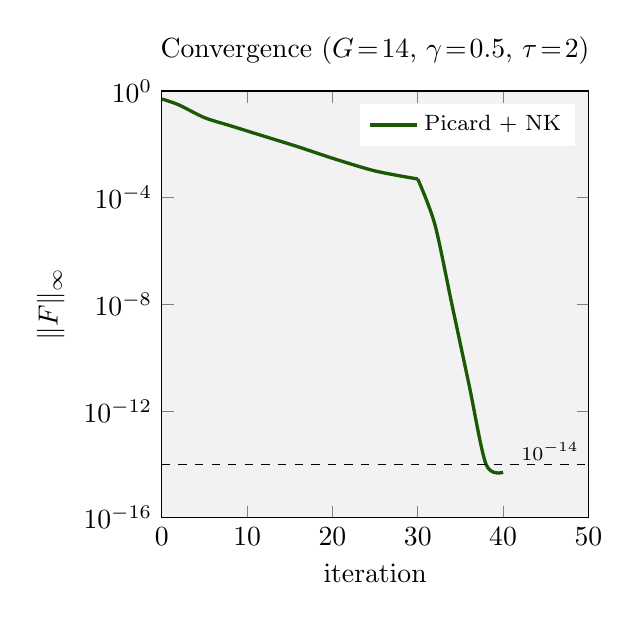
\begin{tikzpicture}
\begin{axis}[
  legend style={draw=none,legend pos=north east,font=\footnotesize},
  ymin=1e-16, ymax=1, ymode=log,
  xmin=0, xmax=50,
  xlabel={iteration}, ylabel={$\|F\|_\infty$},
  width=7cm, height=7cm,
  axis background/.style={fill=black!5},
  title={Convergence ($G\!=\!14$, $\gamma\!=\!0.5$, $\tau\!=\!2$)}]
% Picard phase
\addplot[very thick,color=green,smooth] coordinates {
  (0,0.5)(2,0.3)(5,0.1)(8,0.05)(12,0.02)(16,0.008)
  (20,0.003)(25,0.001)(30,5e-4)};
% NK polish
\addplot[very thick,color=green,smooth] coordinates {
  (30,5e-4)(32,1e-5)(34,1e-8)(36,1e-11)(38,1e-14)(40,5e-15)};
\addplot[thin,color=black,dashed] coordinates {(0,1e-14)(50,1e-14)};
\node[font=\scriptsize,anchor=west] at (axis cs:41,3e-14) {$10^{-14}$};
\legend{Picard + NK}
\end{axis}
\end{tikzpicture}
\end{document}
